\section{En busca de la eficiencia}
\subsection{Algoritmos de ordenamiento}
Los \textbf{algoritmos de ordenación} son un conjunto de instrucciones que toman un arreglo o lista como entrada y organizan los elementos en un orden particular.
Las ordenaciones suelen ser numéricas o una forma de orden alfabético (o lexicográfico), y pueden ser en orden ascendente (AZ, 0$-$9) o descendente (ZA, 9$-$0).

Estos algoritmos son fundamentales dado que permiten reducir la tarea de ordenar datos a una tarea más simple y eficiente. Estos algoritmos tienen aplicaciones directas en algoritmos de búsqueda, algoritmos de bases de datos, algoritmos de estructura de datos y muchos más.

Para la creación de este programa se requiere la ordenación de diferentes listas enlazadas (Listas de usuarios, de bandas, de géneros y comentarios) bajo criterios tanto numéricos como lexicográficos.

Inicialmente se planteó el uso del algoritmo Bubble Sort o \textbf{Ordenamiento por intercambio} el cuál, compara pares de elementos adyacentes y los intercambia si están en el orden incorrecto. Repite este proceso hasta que todos los elementos estén ordenados. Este algoritmo es fácil de implementar pero su eficiencia es bastante baja, con una complejidad temporal de $O(n^2)$. Dado que su rendimiento empeora conforme crece el tamaño de la lista, se consideró que no era adecuado para este proyecto, donde se manejan conjuntos de datos más grandes.
\begin{figure}[H]
    \centering
    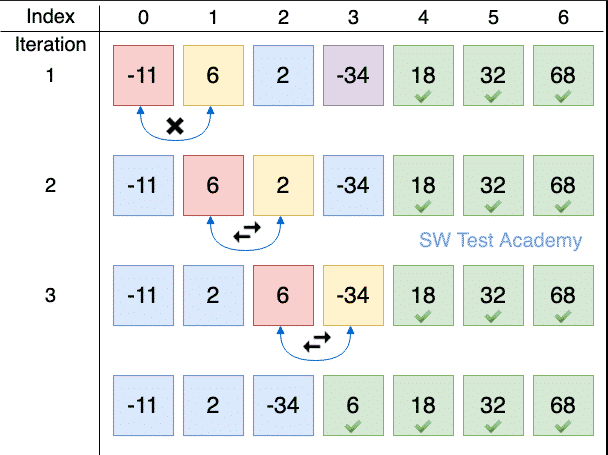
\includegraphics[width=0.5\textwidth]{./src/images/BubbleSort.png}
    \caption{Bubble Sort}
    \label{fig:BubbleSort}
\end{figure}
\newpage
Por otro lado el algoritmo Merge Sort o \textbf{Ordenamiento por Mezcla} divide el conjunto de elementos en subconjuntos más pequeños, los ordena por separado y luego los fusiona para obtener un conjunto ordenado más grande. Este algoritmo utiliza la estrategia de ``divide y vencerás'', lo que le da una eficiencia mucho mayor que Bubble Sort, con una complejidad temporal de $O(n \log n)$. Dado que el proyecto implicaba manejar (posiblemente) grandes volúmenes de datos, se optó por Merge Sort debido a su mejor comportamiento en términos de rendimiento.
\begin{figure}[H]
    \centering
    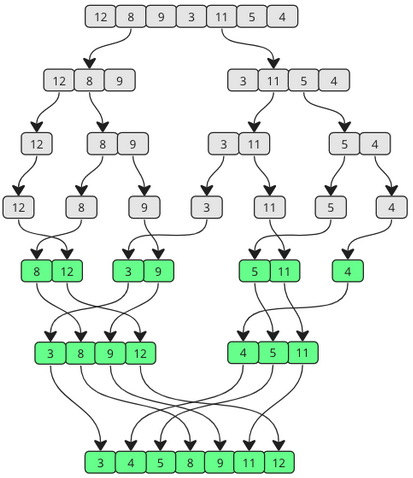
\includegraphics[width=0.5\textwidth]{./src/images/MergeSort.png}
    \caption{Merge Sort}
    \label{fig:MergeSort}
\end{figure}
\newpage
\subsection{JSON}
\textbf{JSON} es un formato de intercambio de datos utilizados para almacenar e intercambiar información estructurada de manera legible. Es ampliamente usado para la transferencia de datos entre servidores y clientes.
\subsubsection*{¿Para qué se utiliza un archivo JSON?} % Esto sería un subtítulo
\textbf{JSON} almacena información en forma de pares clave-valor y es utilizado principalmente para transferir datos estructurados. Un archivo JSON puede contener diferentes tipos de datos, como cadenas de texto, números, objetos, arreglos, valores booleanos y null, como se muestra en la figura \ref{fig:json}
\begin{figure}[H]
    \centering % Para que aparezca centrada
    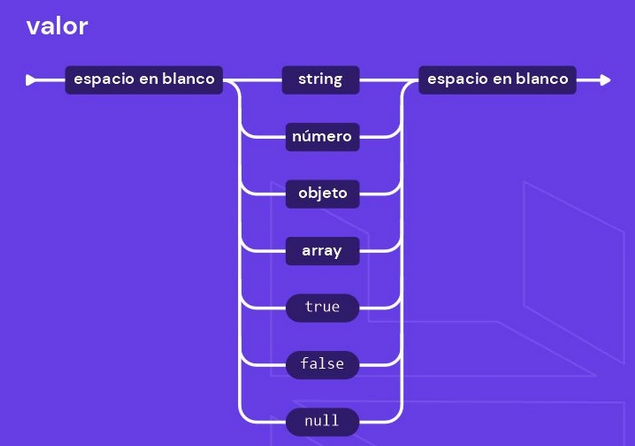
\includegraphics[width=0.5\textwidth]{./src/images/json.png} % Esta linea incluye la imagen
    \caption{Diagrama json} % Este es el mensaje que acompaña la imagen
    \label{fig:json} % Esta es la referencia a la imagen
\end{figure}
En el estracto de código \ref{lst:json} se muestra un ejemplo de un archivo JSON que contiene información sobre un usuario perteneciente a \loopweb
\begin{lstlisting}[language=C, caption={Ejemplo de .json}, label={lst:json}]
{
  "userName": "Alice",
  "age": 18,
  "nationality": "Spain",
  "genres": [ "rock", "pop" ],
  "artists": [ "rihanna", "ladyGaga" ],
  "description": "Amante de los festivales de musica.",
  "friends": [ "Bob", "Carol", "Mallory" ]
}
\end{lstlisting}

\newpage
\subsubsection*{¿Cómo utilizar JSON en C?}
Para trabajar con archivos .json en C, es necesario utilizar librerías externas. Algunas opciones son:
\begin{enumerate}
    \item Jansson
    \item Json-c
    \item cjson
\end{enumerate}
En este caso, se usará la librería \href{https://github.com/akheron/jansson}{Jansson}.

Jansson es una librería de C para trabajar con datos JSON, simple, sin dependencias externas y con documentación completa.

Algunas de las funcionalidades más importantes de Jansson son:
\begin{enumerate}
    \item \textbf{json\_error\_t}: Tipo de dato para almacenar errores durante la lectura de un archivo JSON.
    \begin{lstlisting}[language=C, caption={json\_error\_t}]
        json_error_t error;
    \end{lstlisting}
    \item \textbf{json\_t}: Tupo de dato para unobjeto JSON, siempre a través de un puntero.
    \begin{lstlisting}[language=C, caption={json\_t}]
        json_t *materias_json = json_object_get(alumnos_json,"materias");
    \end{lstlisting}
    \item \textbf{json\_loadf()}: Carga el contenido de un archivo JSON en una variable de tipo json\_t.
    \begin{lstlisting}[language=C, caption={json\_loadf}]
        json_t *json = json_loadf(archivo,0,&error);
    \end{lstlisting}
    \item \textbf{json\_object\_get()}: Accede a los valores de un objeto JSON.
    \begin{lstlisting}[language=C, caption={json\_object\_get}]
        json_object_value(alumnos_json,"nombre");
    \end{lstlisting}
    \item \textbf{json\_string\_value()}: Extrae el valor de una cadena de texto en JSON.
    \begin{lstlisting}[language=C, caption={json\_string\_value}]
        json_string_value(json_object_value(alumnos_json,"nombre"));
    \end{lstlisting}
    \newpage
    \item \textbf{json\_integer\_value()}: Extrae el valor de un entero de un objeto JSON.
    \begin{lstlisting}[language=C, caption={json\_integer\_value}]
        json_integer_value(json_object_value(alumnos_json,"edad"));
    \end{lstlisting}
\end{enumerate}

La utilización de arhcivos JSON para el almacenamiento de la información de este programa es crucial para que la información sea sencilla de almacenar y eficiente de leer, permitiendo no cargar toda la información del programa en cada acción sino cargar \textbf{solo lo necesario} en| cada momento.